% Software License Agreement
%
% Author    Chris Bogdon <cbogdon@clearpathrobotics.com>
% Copyright (c) 2015, Clearpath Robotics, Inc., All rights reserved.
%
% Redistribution and use in source and binary forms, with or without modification, is
% not permitted without the express permission of Clearpath Robotics.


\documentclass[]{clearpath-latex/clearpath-manual}
\graphicspath{{gen/}}
\usepackage{multirow}
\usepackage{gensymb}
\usepackage{dcolumn}
\usepackage{colortbl}
\usepackage{array}
\usepackage{hyperref}
\usepackage{fancyhdr}
\pagestyle{fancyplain}
\lfoot{Rev. 1.1.3}
\rfoot{Ridgeback}
\lhead{}
\chead{}
\rhead{}
\renewcommand{\headrulewidth}{0pt}


\begin{document}

\manualcover{cover-page.pdf}
\tableofcontents

\section{Introduction}
Clearpath Robotics Ridgeback is a rugged, indoor omnidirectional platform designed to move manipulators and other heavy payloads with ease and precision. This guide contains information about the setup, safe operation, and maintenance of your Ridgeback unmanned omnidirectional platform.

\subsection{What's Included}

Included with each Ridgeback are the following:

\begin{itemize}[nolistsep]
  \item 1x Ridgeback Omnidirectional Robotic Platform
  \begin{itemize}
    \item{Integrated Core i5 Mini-ITX Computer}
    \item{Hokuyo UST-10LX LIDAR (forward facing)}
    \item{User Integration Area with power, Ethernet, and USB connectivity}
    \item{24V Lead Acid Battery Pack}
    \item{Onboard Battery Charger}
  \end{itemize}
  \item 1x Sony Bluetooth controller
  \item 1x Ridgeback User Manual
\end{itemize}

\subsection{Expansions}

To expand the capabilities of Ridgeback, consider the following packages offered by Clearpath Robotics:

\subsubsection{LIDAR Upgrades}

A rear-facing LIDAR is available, which when combined with the standard front-facing LIDAR, offers Ridgeback a full 360 degree view of the environment.

Additionally, either or both of the LIDARs may be upgraded to our premium option, the SICK LMS111, offering expanded range and accuracy to your mapping and localization activities.

\subsubsection{Baxter Package}

The Baxter Package includes an adjustable podium mount, power system tie-ins and communication for Baxter. Easily coordinate behaviours between Ridgeback and Baxter with full ROS, Gazebo Simulator, RViz, and MoveIT! Motion planner support.

The package includes the following elements:

\begin{itemize}[nolistsep]
	\item Baxter Mounting Podium
	\item 120/240V VAC power inverter
\end{itemize}

Note that the integration between Ridgeback and Baxter is a quick and painless process. It can easily be carried out by the user if you have a pre-existing Baxter which you'd like to make mobile with Ridgeback. Just be sure to order the power inverter option and you'll be good to go.

\subsubsection{Universal Robot Manipulation Packages}

The UR packages include mechanical mounting, integrated UR controller, power and communications for the selected Universal Robotics robot arm. Also included are a Robotiq 3-Finger gripper and a force torque sensor. Easily coordinate behaviours between Ridgeback and UR5 with full ROS, Gazebo Simulator, RViz and MoveIT! Motion planner support.

The following elements are included with the UR packages:

\begin{itemize}[nolistsep]
	\item UR5 or UR10 robotic arm
	\item 3 Finger 85 Robotiq gripper
	\item Robotiq FT 150 force-torque sensor
	\item BumbleBee stereo camera
	\item FLIR PTU D46-17 pan-tilt unit
\end{itemize}


\pagebreak[4]
\subsection{Hardware Overview}

Please see \autoref{ridgeback_overview} for a view of some of Ridgeback's key external-facing features.

\begin{figure}[h]
  \centering
  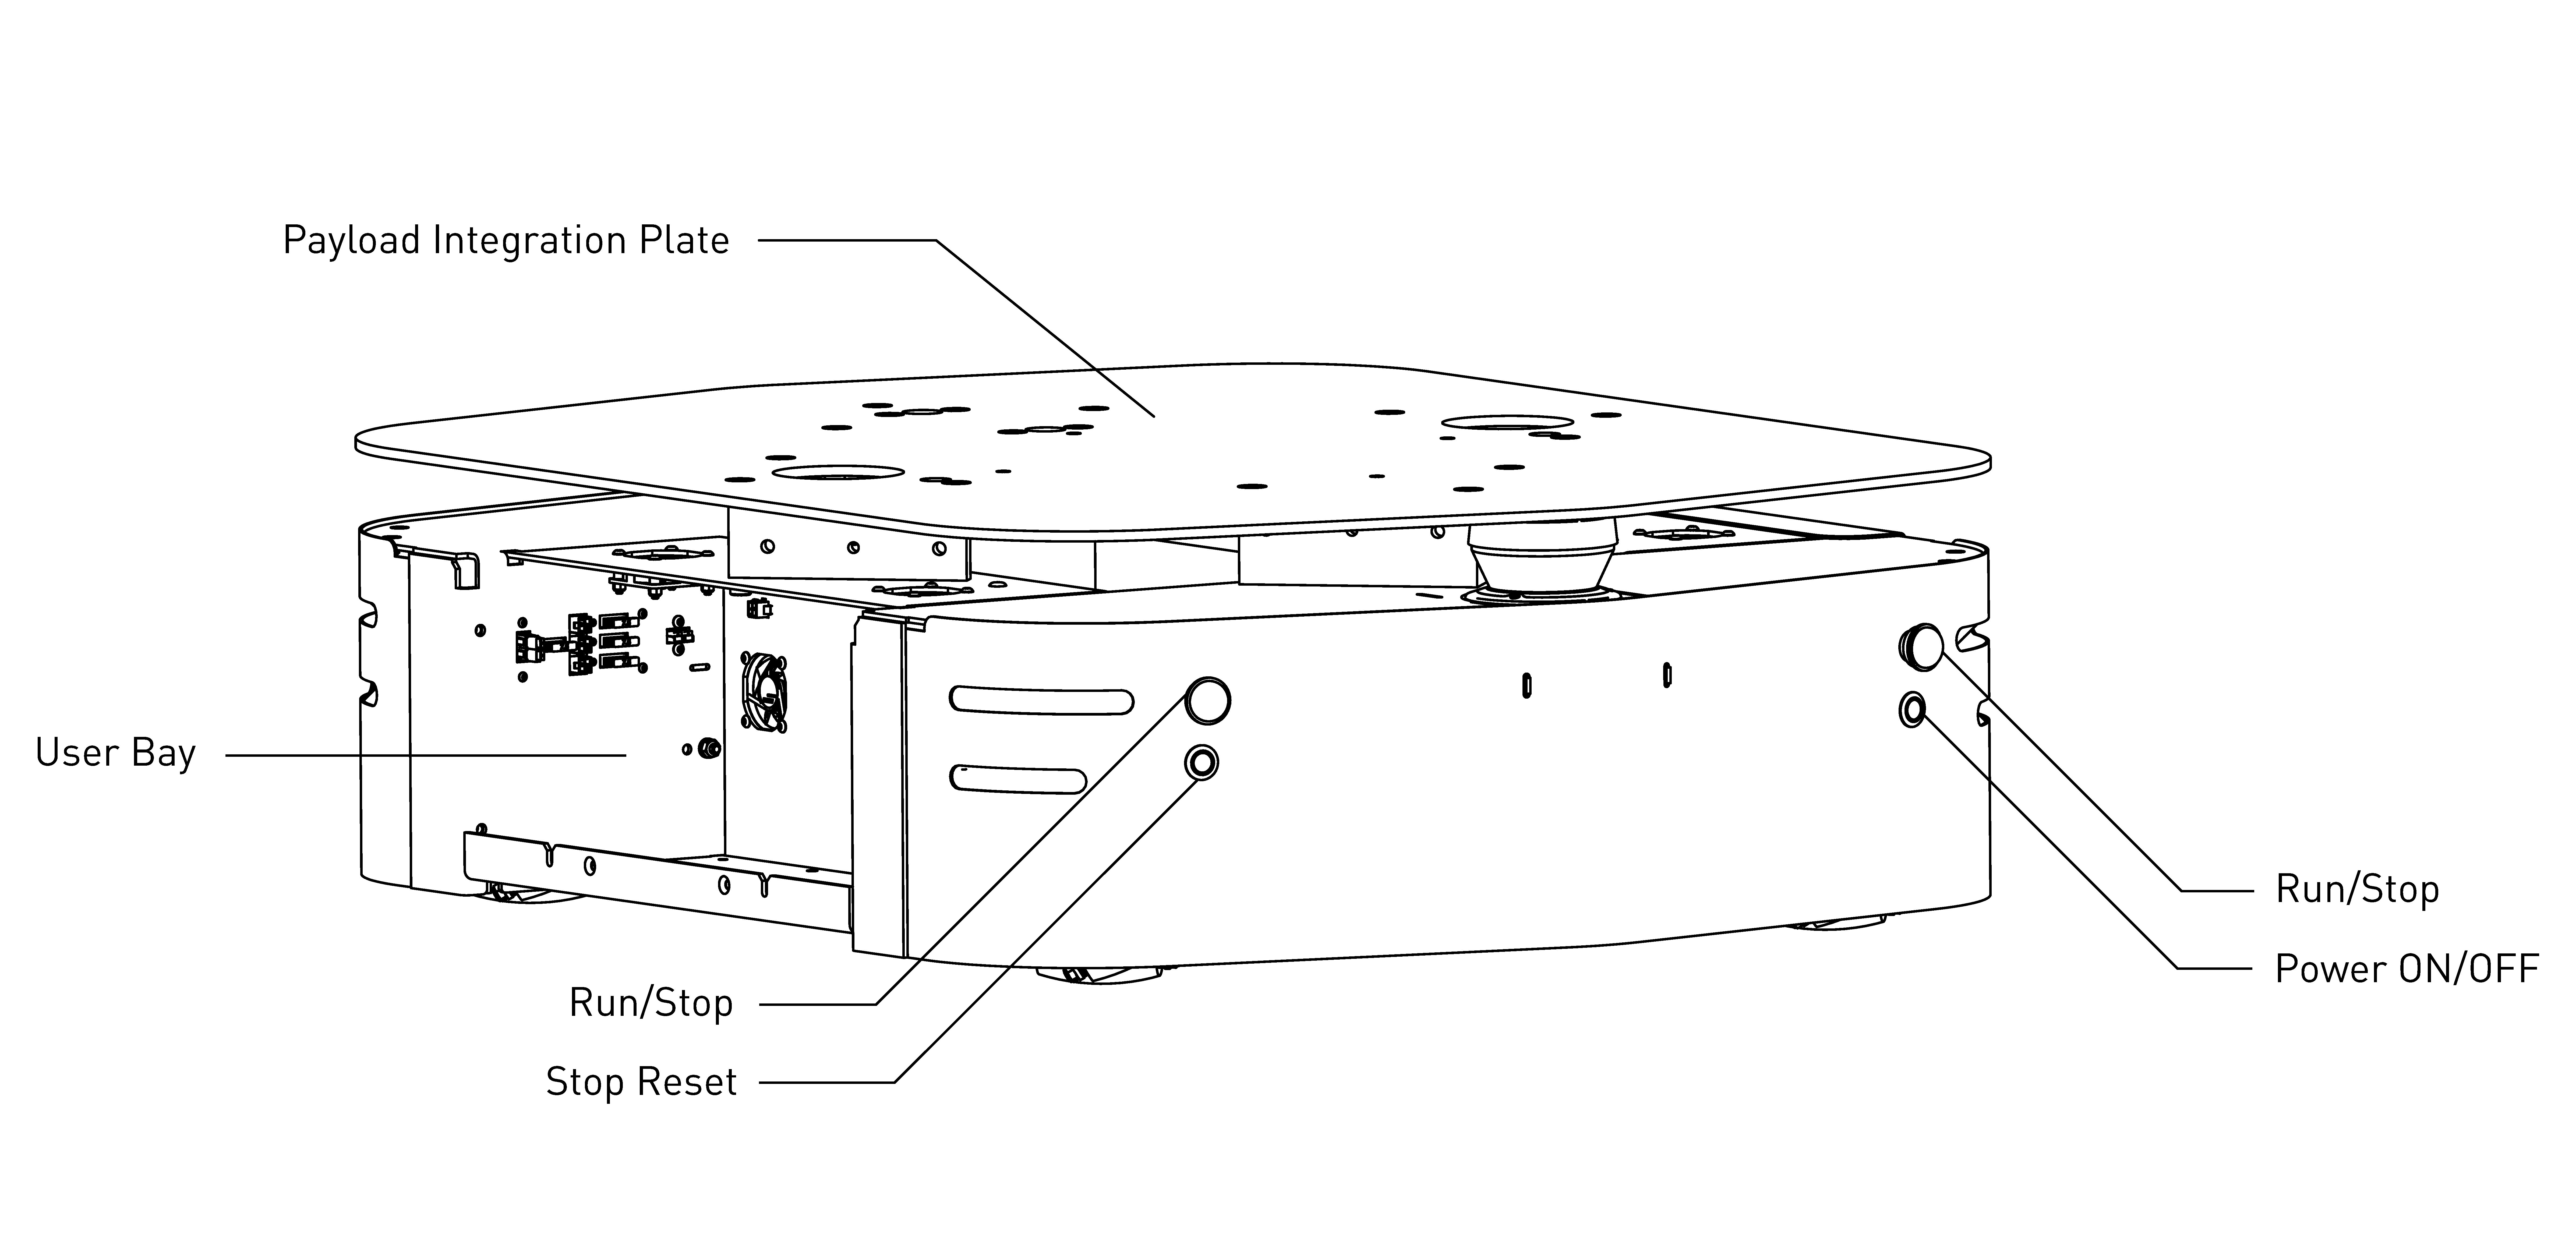
\includegraphics[width=1\linewidth]{Ridgeback_Rear_Drawing_Labeled.pdf}
  \caption{Ridgeback Hardware Overview}
  \label{ridgeback_overview}
\end{figure}

The two yellow side panels may be removed by sliding them upward and away from the main chassis. The starboard-side bay contains Ridgeback's integrated computer, network switch, and main microcontroller PCB. Under most ordinary circumstances, you should not need to access this bay. The port-side bay is the user bay, discussed below on page \pageref{userbay}


\pagebreak[4]
\subsubsection{Buttons}

There are four push buttons located on the back of the Ridgeback: The two red mushroom stop buttons, the stop reset button below the port side stop button, and the power ON/OFF button below the starboard side stop. On the front of the robot, there are another two red mushroom stop buttons.  These are described further in \autoref{rearbuttons}.

\bgroup
\def\arraystretch{1.2}%
\begin{table}[h]
	\centering
	\begin{tabular}{>{\columncolor{lightgrey}}>{\raggedright}m{.20\textwidth} p{.75\textwidth}} \hline

	Power ON/OFF & Turns Ridgeback on or off. Note that the power button is a soft, momentary switch: to shut Ridgeback down, press and release it, and when the onboard PC has completed a safe power-down, the robot itself will also de-power. \\ \hline

	Stop (x4) & Stops Ridgeback by placing the four integrated motor drivers into an electrical reset condition. This is intended as a backup option for immobilizing Ridgeback when autonomy software malfunctions or commands unintended motion. The stop buttons have a mechanical latch, which can be released by twisting the latched button.

	If you have a wireless e-stop, pendant, or other stop-asserting hardware you'd like to integrate with Ridgeback, a breakout header is supplied on the main microcontroller PCB. For details on this interface, please contact Clearpath Robotics. \\ \hline

	Stop Reset & Clears the electrically-enforced stop latch, allowing Ridgeback to run again after it has been stopped via one of the stop buttons. Note that the mushroom button's mechanical latch must be cleared before the electrical reset can have any effect. \\ \hline
	\end{tabular}
\newline
\caption{Ridgeback Rear Buttons}
\label{rearbuttons}
\end{table}
\egroup


\pagebreak[4]
\subsubsection{Body Lights}

Ridgeback includes eight RGB body lights, stacked in a pair on each corner of the chassis. These lights express system status according to \autoref{bodylights}, but in the absence of one of the low-level conditions, they can be commanded from ROS to display indications from autonomy or other higher-level software.

See \url{http://wiki.ros.org/ridgeback_base} for information on commanding the body lights.

\bgroup
\def\arraystretch{1.2}%
\begin{table}[h]
	\centering
	\begin{tabular}{>{\columncolor{lightgrey}}>{\raggedright}m{.25\textwidth} p{.7\textwidth}} \hline

	Solid red & The MCU is not in contact with the computer. That is, the rosserial connection is not active. This condition will be seen briefly on startup while Ridgeback's computer is booting up. If it persists, or is seen after initialization, either the base node on the PC has crashed, the network switch has failed, or a serious MCU error has occurred. If you suspect one of these conditions, please contact support. \\ \hline

	Red flashing & Stop circuit is broken. Twist the mushroom buttons to ensure that they are unlatched, and check any external stop hardware, if present. \\ \hline

	Yellow corner flashing & All stops are closed but not reset, the stop loop is now only electrically latched. Press the stop reset button to enable full operation. \\ \hline

  Flashing yellow & Motor drivers not yet ready to drive. The motors have a brief initialization sequence which must complete after a stop condition clears before they are ready to drive. If this condition persists, please contact support. \\ \hline

  Fading green & Charger is connected, Ridgeback's battery is charging. Note that the battery can also be charged with the platform off. This indication will only be seen if the charger is connected while Ridgeback is powered up. \\ \hline

  Headlights/taillights & When Ridgeback is ready to drive, the front will change from red to white. The intensity of the head and tail lights will increase slightly when actually in motion. This is the status which may be overridden by publishing your own light patterns to the cmd\_lights ROS topic. \\ \hline

	\end{tabular}
\newline
\caption{Ridgeback Body Light Indications}
\label{bodylights}
\end{table}
\egroup


\pagebreak[4]
\subsubsection{User Bay}\label{userbay}

The User Bay provides access to the User Power panel, as well as USB and Ethernet ports, and additional space for stowing user equipment.  The electrical panel can be used to power your payloads. The USB3 ports are connected directly to the onboard PC, and the ethernet ports connect to the onboard network switch. To connect a device to the onboard network, it's suggested to give it a static IP in the \lstinline{192.168.131.x} subnet and this cannot be changed since the MCU is statically set to \lstinline{192.168.131.2} and expects the computer to be at \lstinline{192.168.131.1}.  Avoiding IPs in use by the following pre-existing devices:

\bgroup
\def\arraystretch{1.2}%
\begin{table}[h]
	\centering
	\begin{tabular}{>{\columncolor{lightgrey}}>{\raggedright}m{.3\textwidth} p{.65\textwidth}} \hline

	192.168.131.1 & Onboard PC (both ports, br0 network interface). \\ \hline

	192.168.131.2 & Ethernet-connected MCU. \\ \hline

	192.168.131.14 & Front-facing LIDAR. \\ \hline

	192.168.131.13 & Rear-facing LIDAR (optional). \\ \hline

	\end{tabular}
\newline
\caption{Ridgeback Onboard Network Devices}
\label{netdevs}
\end{table}
\egroup

For more information on electrical integration, please see \autoref{electrical} on page \pageref{electrical}.


\subsubsection{Payload Integration Plate}

The Payload Integration Plate provides a robust foundation for mounting payload structures such as Baxter, UR5/UR10 manipulation arms, or any other combination of sensors and manipulators.   For more information and guidance on mounting payload structures on top of Ridgeback, please refer to \autoref{mechanical} on page \pageref{mechanical}.


\pagebreak[4]
\subsection{Technical Specifications}

Key specifications of Ridgeback are shown in \autoref{systemspecs}.

\bgroup
\def\arraystretch{1.2}%
\begin{table}[h]
	\centering
	\begin{tabular}{>{\columncolor{lightgrey}}>{\raggedright}m{.30\textwidth} p{.70\textwidth}} \hline

	External Dimensions (L x W x H) & 960 x 793 x 296 mm   (37.7 x 31.1 x 11.6 in) \\ \hline
	Weight & 135 kg (297 Ilbs) \\ \hline
	Obstacle Clearance & 18 mm (0.7 in) \\ \hline
	Max Payload  &  100kg (220 lbs)  \\ \hline
	Max Speed  &  1.1 m/s (3.6 ft/s) \\ \hline
	Drive Configuration &  4 Independently driven omni-directional wheels \\ \hline
	Operating Environment  &  Indoor \\ \hline
	Battery Chemistry & Marine Grade AGM Sealed Lead Acid \\ \hline
	Capacity &  24 V 100 Ah \\ \hline
	Operating Time & 15 hrs with max payload \\ \hline
	Charge Time &  8 Hours approx \\ \hline
	User Power & 5 V, 12 V, 24 VDC (fused at 10A each), option 120 VAC \\ \hline
	Power & 800 W Typical Use, Shore Power Available \\ \hline
	Control Modes & Kinematic control (forward, sideways, rotation), individual wheel velocities \\ \hline
	Feedback & Encoders, Onboard IMU \\ \hline
	Communication &  Ethernet, USB 3.0, RS 232 \\ \hline
	Drivers and APIs  &  ROS Indigo, Gazebo, Navigation Support, MoveIt! \\ \hline

	\end{tabular}
\newline
\caption{Ridgeback System Specifications}
\label{systemspecs}
\end{table}
\egroup




\section{Getting Started}

The first step is to power up your Ridgeback and have some fun driving it around! If you’re just opening up the shipping crate, you can unfold the ramp, and remove the ratchet straps which secure Ridgeback during shipping.

Press the power button on the back of Ridgeback. Once the body lights are flashing red, clear the two stop buttons (if necessary), and press the blinking red stop reset button. In a moment, the platform should go to solid red lights in back, and solid white in front.

Press the PS button on the Sony Bluetooth controller to sync the controller to Ridgeback. Once the \#1 LED on the top of the controller goes solid, you’re paired and ready to drive. Hold the L1 trigger button, and pull the left thumbstick down. This should cause Ridgeback to back slowly down the ramp onto level ground. Once there, you can experiment with the teleop controls: left thumbstick to translate in X and Y, and right thumbstick to rotate on the spot.

If you’re not seeing any action, check Contact on \autoref{contact} to get in touch with support.

\subsection{Wireless Access}

To get Ridgeback connected to your local wifi, you must first access the internal computer using a wired connection. Open the User Bay, and connect to one of the the network ports with a standard ethernet cable. Now, set your laptop’s ethernet port to a static IP such as \lstinline{192.168.131.51}, and connect via SSH to \lstinline{administrator@192.168.131.1}. The default password is \lstinline{clearpath}.

Once connected via wire, execute \lstinline{connmanctl} to enter the command line interface for Connman, from which you can configure Ridgeback to either join an existing network, or supply its own standalone access point. An example session to connect to an existing network:

\begin{lstlisting}
connmanctl> enable wifi
connmanctl> scan wifi
connmanctl> services
connmanctl> agent on
connmanctl> connect wifi_123456_123456789123456789_managed_psk
\end{lstlisting}

After the \lstinline{connect} line, connman will prompt you for your network's passphrase. Once connected, connman will remember and attempt to reconnect on successive power-ons.

\subsection{Remote ROS Connectivity}

Now that Ridgeback is on the wireless network, you can access it via SSH or as a remote ROS master. Note that in the default configuration, the background ROS process running on Ridgeback launches with the \lstinline{robot_upstart} package, which is configured to set the \lstinline{ROS_HOSTNAME} environment variable to the Ridgeback PC's hostname.

If your network resolves hostnames properly, connecting should be a matter of executing the following two lines in your desktop (or sourcing a script containing these lines):

\begin{lstlisting}
export ROS_MASTER_URI=http://cpr-ridgeback:11311  # Your robot's hostname
export ROS_IP=10.25.0.102                         # Your computer's wireless IP address
\end{lstlisting}

If your network doesn't resolve hostnames, you may need to add the following line to your \lstinline{/etc/hosts} file:

\begin{lstlisting}
10.25.0.101 cpr-ridgeback                         # The robot's wireless IP address.
\end{lstlisting}

Once you believe everything is set up correctly, try running \lstinline{rostopic list}, which will verify that your machine can see the robot's ROS master, and \lstinline{rostopic echo /mcu/status}, which will verify that the robot PC can see your machine in order to stream topics to it.

Please contact Clearpath Support if guidance is required in selecting and executing a remote access strategy.
For more general details on how ROS works over TCP with multiple machines, please see:

\url{http://wiki.ros.org/ROS/Tutorials/MultipleMachines}

For help troubleshooting a multiple machines connectivity issue, see:

\url{http://wiki.ros.org/ROS/NetworkSetup}

\subsection{Visualizing Ridgeback}

To command or observe Ridgeback from your desktop computer, first set up a basic ROS installation.  See the following page for details:

\url{http://wiki.ros.org/indigo/Installation/Ubuntu}

When your ROS install is set up, install the Ridgeback desktop packages:

\begin{lstlisting}
sudo apt-get install ros-indigo-ridgeback-desktop
\end{lstlisting}

Once your remote access to Ridgeback's ROS master is configured (as above), you can launch rviz, the standard ROS robot visualization tool:

\begin{lstlisting}
roslaunch ridgeback_viz view_robot.launch
\end{lstlisting}

From within rviz, you can use interactive markers to drive Ridgeback, you can visulize its published localization estimate, and you can visualize any attached sensors which have been added to its robot description XML (URDF).

\pagebreak[4]

From your desktop, you can also launch the standard RQT Robot Monitor, which reports the diagnostic output from Ridgeback's self-monitoring capabilities, as shown in \autoref{robotmonitor}:

\begin{lstlisting}
rosrun rqt_robot_monitor rqt_robot_monitor
\end{lstlisting}

\begin{figure}[!htb]
  \centering
  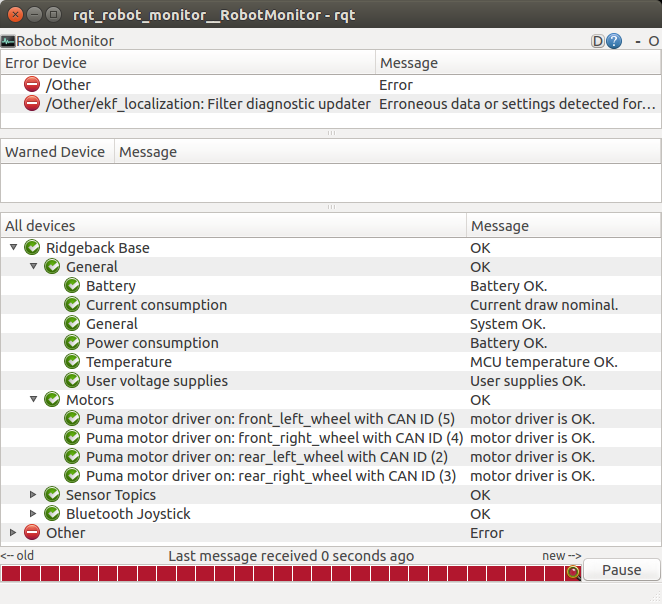
\includegraphics[width=0.75\linewidth]{rqt_robot_monitor.png}
  \caption{Robot Monitor}
  \label{robotmonitor}
\end{figure}


\section{Safety Considerations}

Ridgeback is a powerful, heavy, fast moving robotic platform. Please read the following notices carefully.

\subsection{General Warnings}

Ridgeback is a rugged and high-performance vehicle. For the safety of yourself and others, always conduct initial experiments and software development with the vehicle raised off the ground. Place a wooden crate, a set of sawhorses, a sturdy storage tub, or any other solid flat structure having a height greater than 6 inches under Ridgeback to keep the wheels clear of the ground (“up on blocks”).

When starting out, favor slower wheel speeds. Ridgeback's control loops can accurately maintain velocities as low as 0.1 m/s. Operating at such speeds will give you more time to react if things don’t go quite as you expect.

\subsection{Stop Buttons}

Two red Stop buttons are located on the front and back of Ridgeback. When in Stop mode the Ridgeback will not drive. The commands received during stop are not buffered; Ridgeback will always act on the latest commands received. This means that if the commands are stopped before the Stop button is released, the Ridgeback will not move. If the commands are continued, Ridgeback will move at the speed commanded once the Stop is released.

Always ensure the Stop button is accessible at all times. Avoid mounting payloads that extend over the rear of Ridgeback and would occlude the Stop buttons.

\subsection{Electrical System}

Ridgeback is powered by two lead-acid (PbSO4) deep-cycle AGM batteries, similar to the type found in electric wheelchairs, golf carts, and other vehicles. Ridgeback's battery is capable of delivering 2000W. This gives Ridgeback's motors their great performance, however, it is also enough power to cause severe bodily harm. Always use caution when operating Ridgeback to avoid personal injury or property damage.  To ensure safety, please observe the following precautions:

\begin{itemize}[nolistsep]
	\item Do not tamper with the battery terminals or wiring.
	\item Do not tamper with the fuse panel, except to check and change the fuses, and to connect and disconnect the 	battery plug.
	\item Always replace fuses with the same type and rating to ensure continued protection against risk of fires.
	\item Consult Clearpath Robotics support if you need to service the battery pack.
	\item Do not lay tools or other objects on top of the battery.
	\item Do not move the robot while charging the battery.
	\item Charge the battery only with the integrated charger installed by Clearpath Robotics.
	\item Please dispose of the batteries properly, or return the battery to Clearpath Robotics to do so.
\end{itemize}

\subsection{Lifting and Transport}

\begin{itemize}[nolistsep]
	\item Ensure that Ridgeback's Stop button is engaged when transporting short distances and powered off when transporting longer distances
	\item Do not push the robot at more than 0.5 m/s (1.6 ft/s) or damage to the motor controls may occur
\end{itemize}


\section{Payload Integration Guide}

If you want to attach custom hardware to Ridgeback, you will have to take care of mechnical mounting, electrical supply, and software integration.  This section aims to equip you with respect to these challenges.

\subsection{System Architecture}

Like most robotic systems, Ridgeback has an onboard PC coupled to a custom microcontroller board. The microcontroller board handles IO, system and battery monitoring, and provides an interface to the CAN-controlled motor drivers. See the diagram in \autoref{systemarchitecture} for more details.

\begin{figure}[!htb]
  \centering
  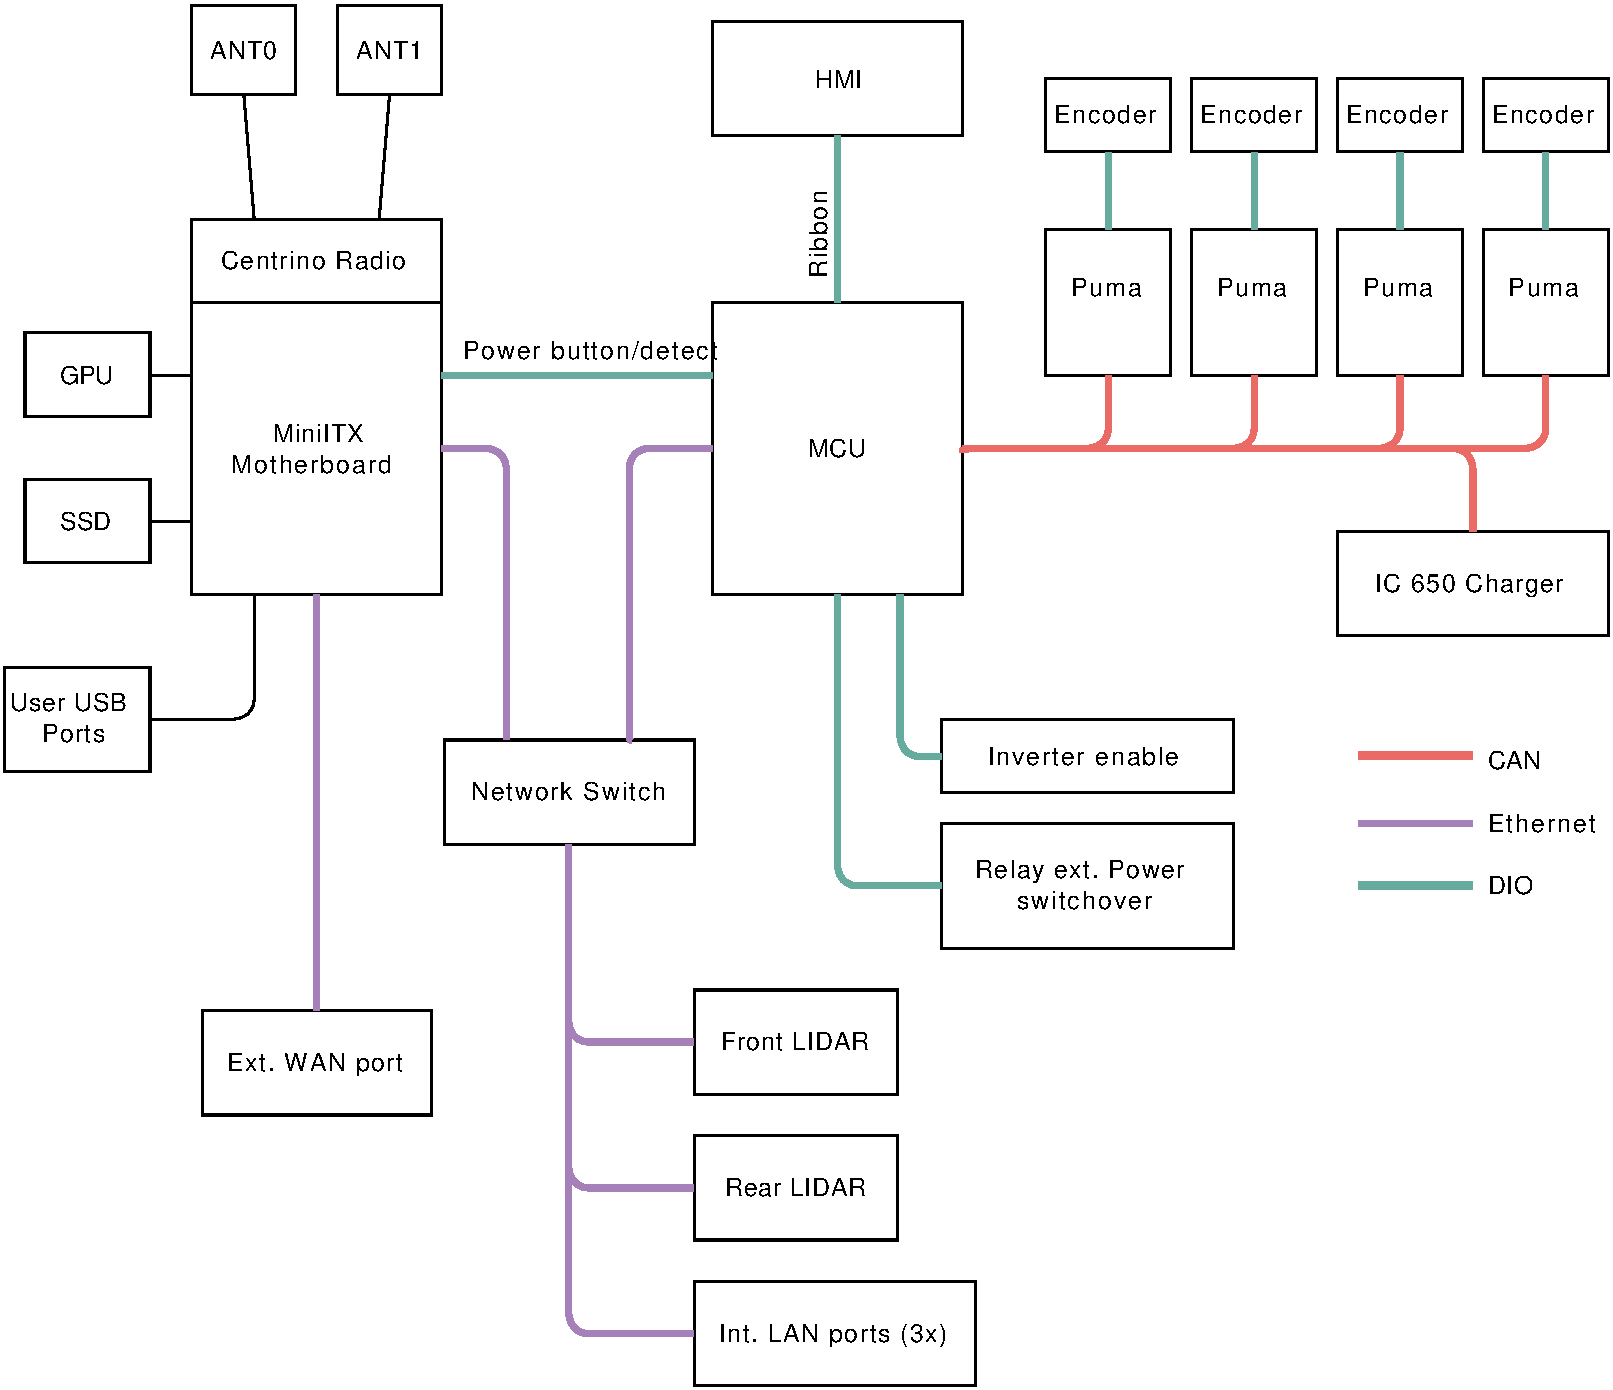
\includegraphics[width=0.75\linewidth]{ridgeback-logic-conn.pdf}
  \caption{System Architecture}
  \label{systemarchitecture}
\end{figure}

\pagebreak[4]
\subsection{Mechanical Mounting}
\label{mechanical}

The payload integration plate can be used to mount external payloads on top of the Ridgeback.   The plate is made of aluminum, which allows Ridgeback to support payloads up to 100 kg (220 lbs).   Ridgeback's battery packs are positioned low in the chassis and slightly rearward of center of the robot to balance the weight distribution when mounting front-facing manipulator payloads. To minimize the possibility of tipping over, payload structures should always be mounted as close to center as possible.

\begin{figure}[!hbt]
  \centering
  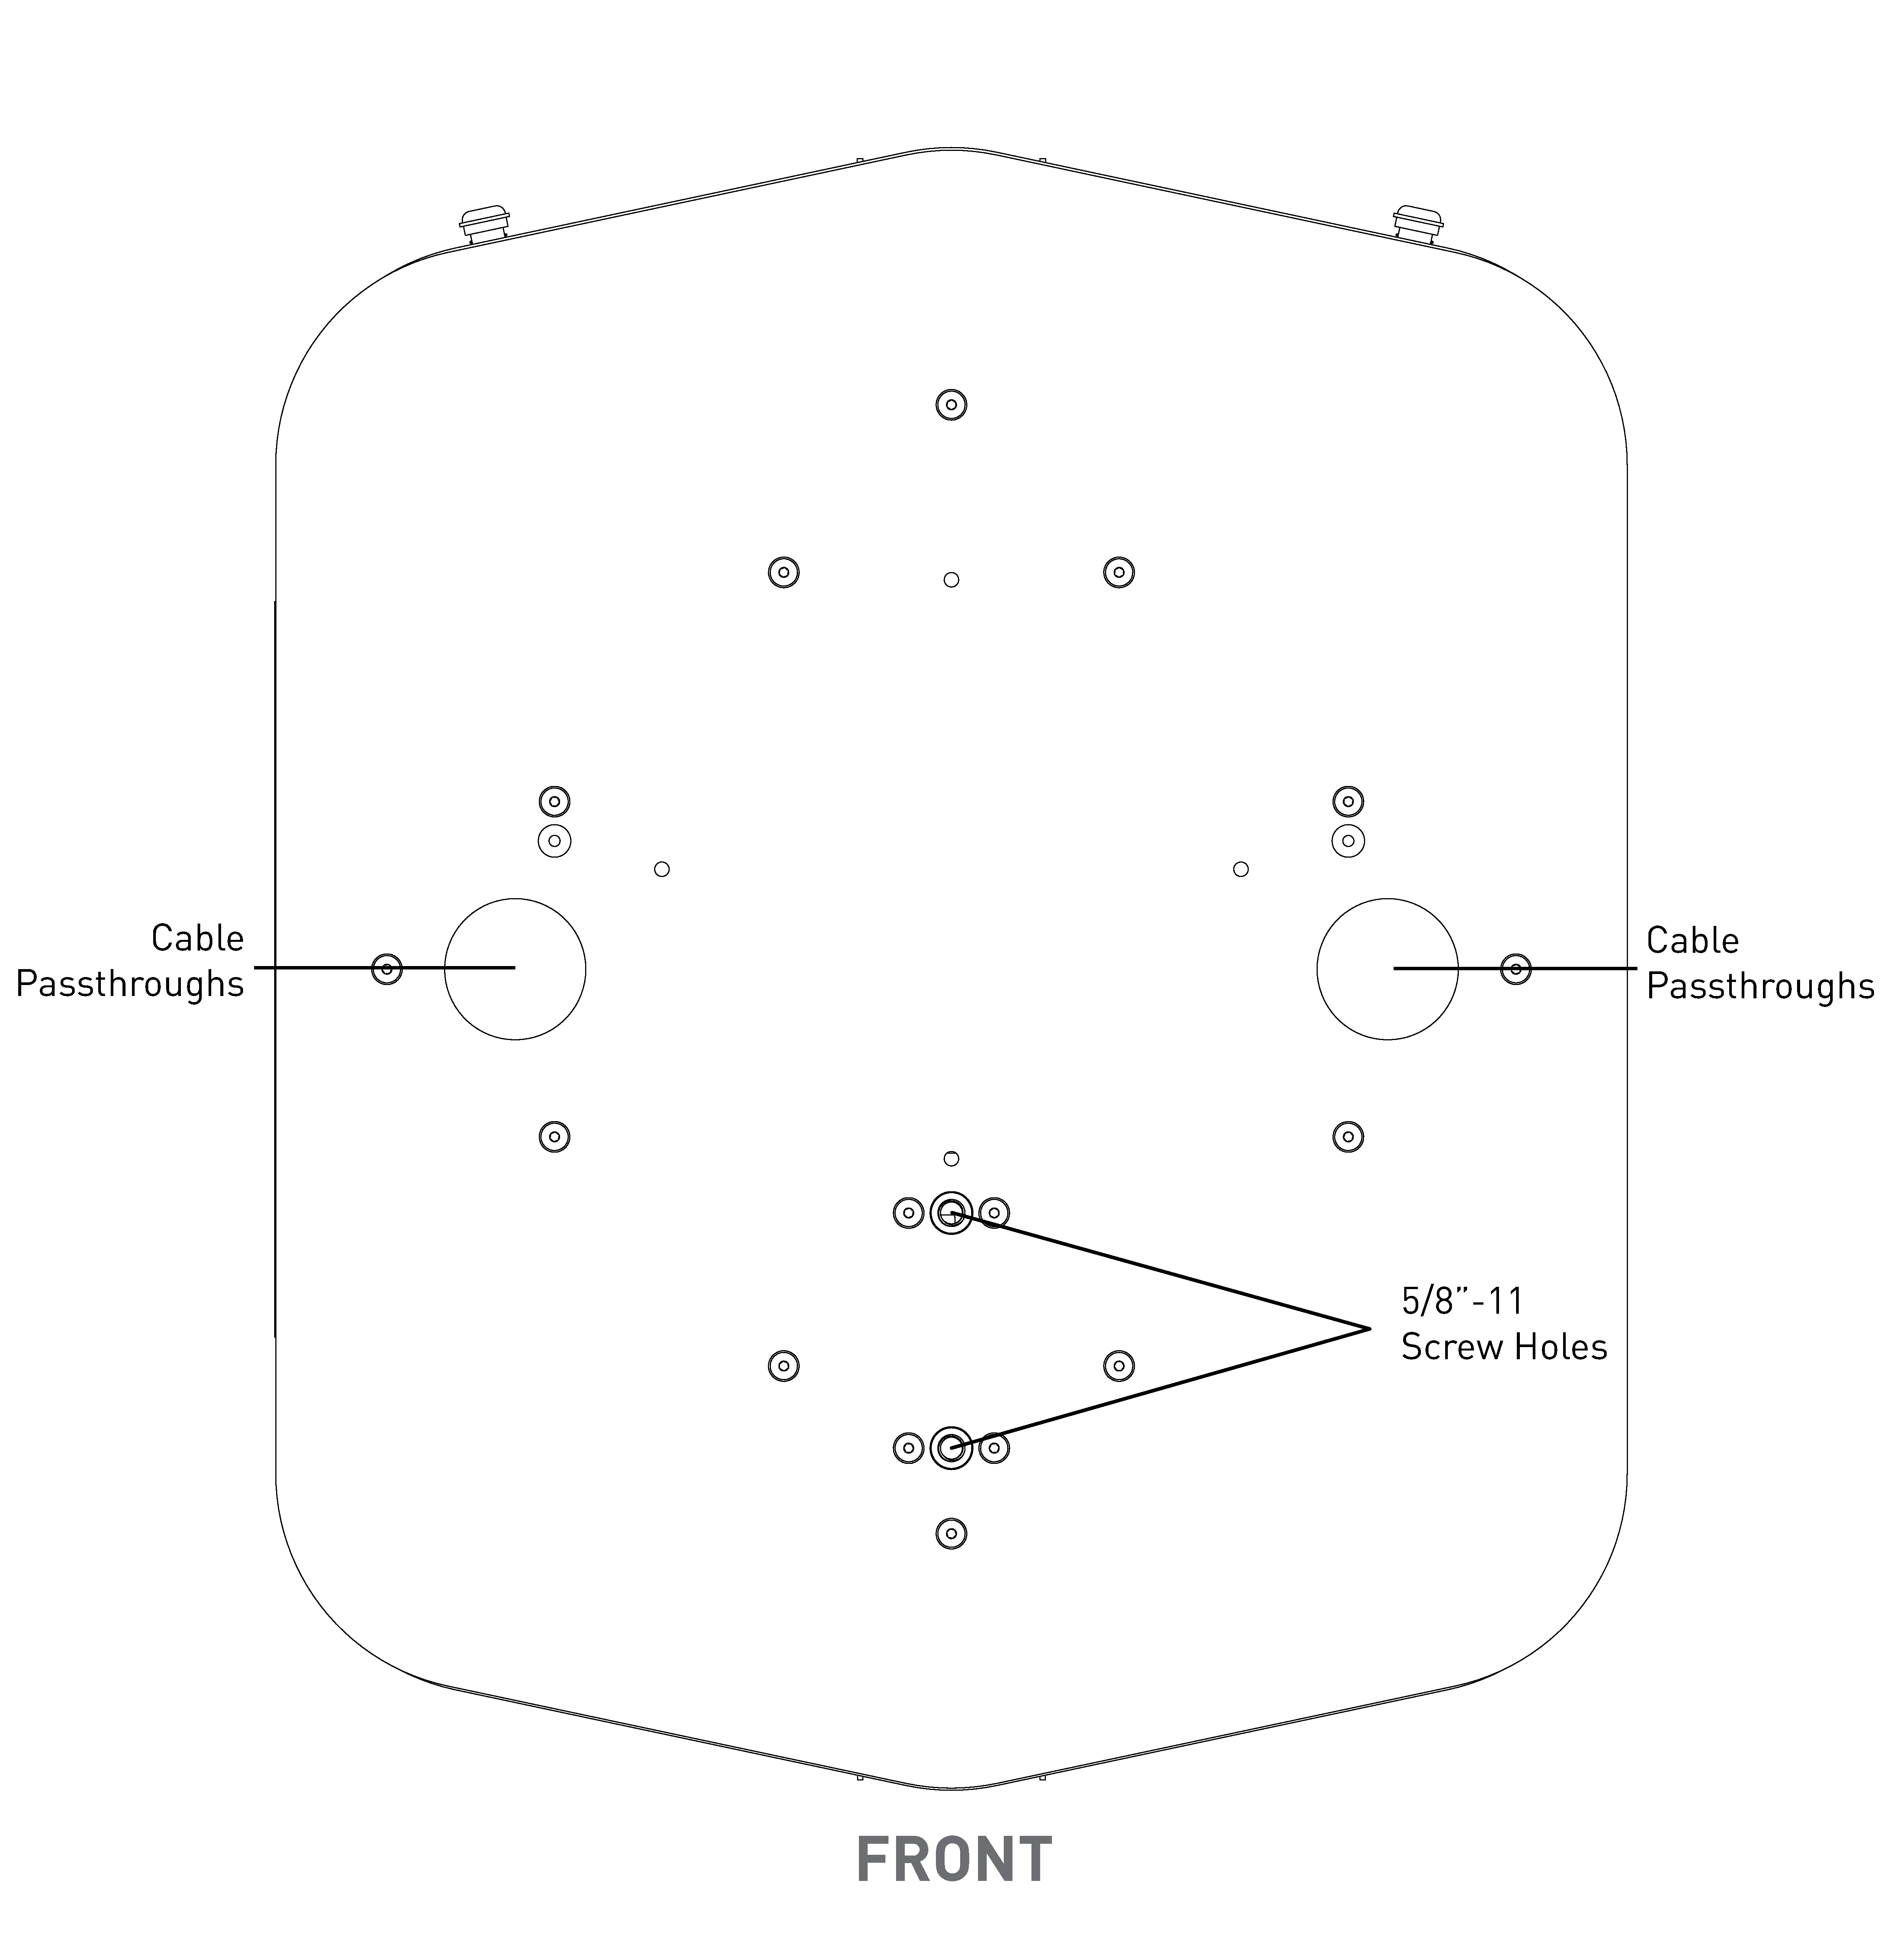
\includegraphics[width=0.75\linewidth]{Payload_Integration_Plate.pdf}
  \caption{Ridgeback Payload Integration}
  \label{payloadplate}
\end{figure}

\subsubsection{Payload Mounting Holes}

Located at the front-end of the mounting plate are two 5/8"-11 screw holes for mounting Baxter, UR5/UR510 manipulator arms, or any other payload structure.  These holes are indicated in \autoref{payloadplate}. If you purchased the Baxter or UR5/UR10 package from Clearpath Robotics, Ridgeback will come with the required hardware adapters to securely mount the payload structures to the plate.

If your payload structure requires additional mounting holes or a different hole configuration, the plate can be removed and additional holes can be drilled.  To remove the mounting plate, simply remove the screws that form the diamond pattern on top of the plate.

\begin{warning}[]
Permanent damage resulting from custom modifications to the mounting plate is not covered under warranty and may not be supported by Clearpath Support.  Please contact our support team if you require assistance or have any questions relating to custom modifications.
\end{warning}

\subsubsection{Cable Passthroughs}

The two larger holes on the left and right side of the plate allow you to pass electrical wires and cables from the mounted payloads into the encolsed User Bay and the PC Bay.  Electrical wires should always pass through the provided plastic grommets to protect against cutting and abrasion.

\pagebreak[4]
\subsection{Electrical Integration}
\label{electrical}

The three white Molex user power receptacles located in the User Bay are capable of supplying 5Vdc, 12Vdc, and unregulated battery voltage (approximately 24Vdc) for powering Ridgeback's payloads. See \autoref{userpower} for an labeled illustration and the pin assignments. The total draw permitted on each rail is 5A. The mating connector for these Molex Mini Fit Jr (tm) receptacles is \lstinline{39-01-2040}, available on Digikey as \lstinline{M3701-ND}. Ensure you select contact appropriate for the gauge of wire used.

\begin{figure}[!h]
  \centering
  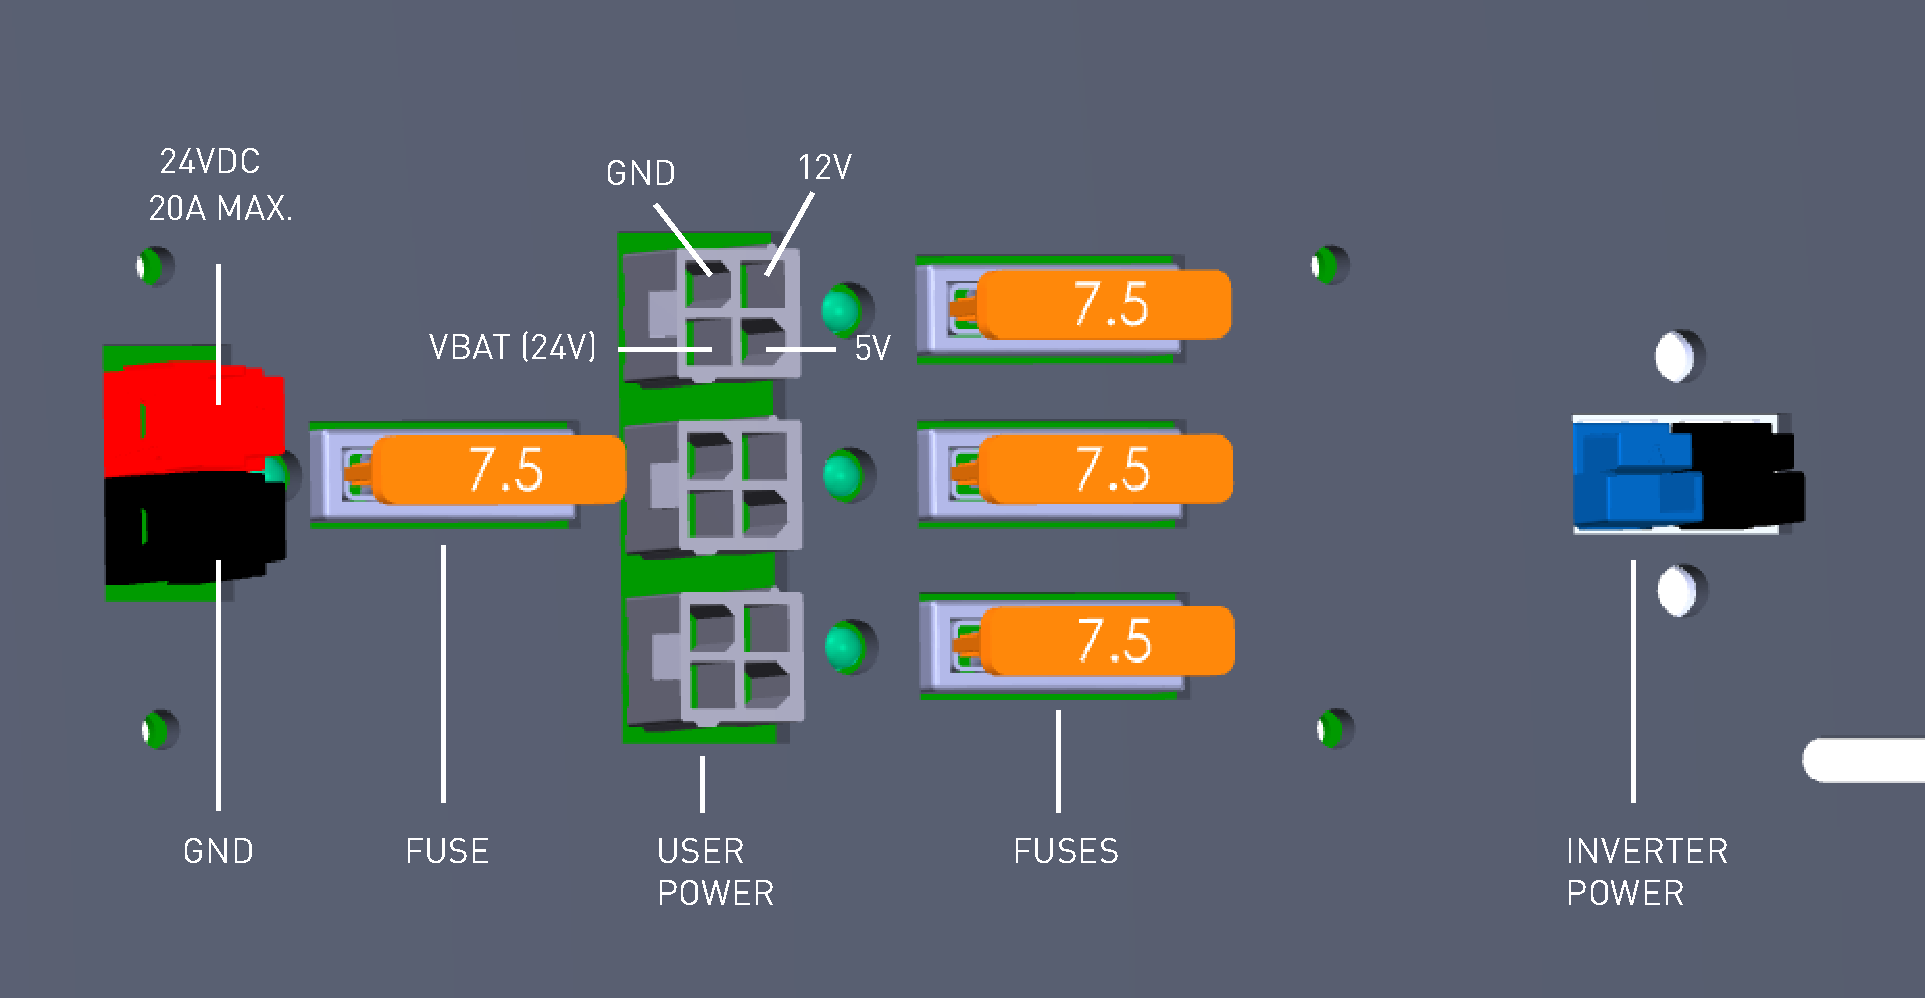
\includegraphics[width=1.0\linewidth]{Ridgeback_UserPower_SOLID.pdf}
  \caption{Ridgeback Power User Panel}
  \label{userpower}
\end{figure}

The single red and black Anderson connector pair provides unregulated battery voltage (approximately 24Vdc) at up to 20-amps peak. The mating parts are Anderson PP45 Power Pole (tm) 1327 (red housing), 1327G6 (black housing) and 261G2-LPBK (contacts.) These components are readily available at \url{http://mouser.com}.

The rails on the User Bay Power board are protected against short circuit by fuses. See the illustration for the fuse locations and purposes.

\begin{warning}[Risk of Fire]
For continued protection against risk of fire, always replace fuses only with those of the same type and rating.
\end{warning}

\begin{warning}[Unregulated Rail]
The unregulated battery output may range from as low as 20Vdc up to 30Vdc or more depending on the state of charge of the battery pack and the electrical loading on the system. Ensure any accessories connected to that rail are able to deal with unregulated battery voltages.
\end{warning}


\subsection{Software Integration}

ROS has a large ecosystem of sensor drivers, some of which include pre-made URDF description and even simulation configurations.  Please see the following page on the ROS wiki for a partial list:

\url{http://wiki.ros.org/Sensors}

For the best experience, consider purchasing supported accessories from Clearpath Robotics for your Ridgeback, which will include simulation, visualization, and driver support.  However, we will happily help you get started with integrating your own devices as well.

\section{Maintenance}

\subsection{Battery \& Charging}

\subsubsection{General}

Ridgeback uses two 8A31DTM Group-31 lead-acid (PbSO4) deep-cycle AGM batteries mounted low in the chassis. They provide an output of 24Vdc (nominal) and 100Ah of capacity and also serve as a ballast to help keep the centre of gravity of the robot low, even with payloads mounted atop it.

Ridgeback has an internal charger. All that is required to charge Ridgeback is to open the User Bay access panel, locate the charger power cord and plug it into any 85-270, 50/60Hz mains outlet. The robot can be turned "on" though we recommend against driving the robot when the battery is charging.

If Ridgeback's batteries need replacement, they're accessible by removing the top-plate and the insulator cover. Before performing any service or maintenance to the robot, the battery pack must be fully disconnected. The batteries weigh approximately 33-kg (73-lbs) each so use all necessary care and caution when lifting the batteries out of the chassis. Please contact Clearpath Robotics regarding replacement batteries.

The battery pack is rugged and designed for the environments into which Ridgeback may be deployed. However, please take note of the following:

\begin{itemize}[nolistsep]
	\item The batteries and/or robot must not be stored or operated above 50◦C or below -20◦C.
	\item If the robot is to be stored for any length of time it should be in a cool, dry location. The batteries should be fully charged and periodically maintained at full charge to ensure a long service life. Ridgeback should not be stored with a low state of charge nor for extended periods of time without top-up charging. The batteries may suffer from "sulfation" which reduces their capacity and lifetime.
	\item Do not allow the batteries to reach a depth of discharge of 80% or more; heed system indications (fading yellow corner lights) that the battery needs charging. Then allow the batteries to achieve full charge before using Ridgeback again.
	\item The batteries must not be punctured or disassembled.
	\item The batteries should be disposed of pursuant to your local regulations regarding electrical and/or hazardous waste
\end{itemize}

\subsubsection{Long-term Storage}

When storing Ridgeback for long periods of time, its important to properly maintain the batteries to fully maximize their life.  Consider one of the following two procedures when placing Ridgeback in long-term storage:

\begin{itemize}[nolistsep]
	\item Fully charge Ridgeback, turn it off and put it into storage.  Once a week, connect power to the charger and allow the charger to top up the battery for an hour or so.
	\item Fully charge Ridgeback, turn it off and put it into storage, but leave the charger connected and powered the enitre time Ridgeback is in storage.  The charger will monitor the battery and will automatically charge it up as needed.
\end{itemize}


Please contact Clearpath Robotics for additional information about Ridgeback's battery pack.


%\subsection{Fuses}
%
%For continued protection against risk of fire, always replace fuses only with those of the same type and rating.
%
%\subsection{Tires}
%
%NEED CONTENT
%
%\subsection{Cleaning}
%
%NEED CONTENT

\section{Contact}
\label{contact}

Clearpath is committed to your success with Ridgeback. Please get in touch with us and we’ll do our best to get
you rolling again quickly: \url{support@clearpathrobotics.com}.

To get in touch with a salesperson regarding Ridgeback or other Clearpath Robotics products, please email
\url{sales@clearpathrobotics.com}.

If you have an issue that is specifically about ROS and is something which may be of interest to the broader
community, consider asking it on \url{answers.ros.org}. If you don’t get a satisfactory response, please ping us and
include a link to your question as posted there. If appropriate, we’ll answer in the ROS Answers context for
the benefit of the community.



\end{document}
